
\section{Funktioner i to variable og differentialregning}

Forklar begrebet funktion i en og to variable, herunder partielt afledede. 

\subsection{Bevis af tangentplanens ligning}

\begin{proofw}

Betragt følgende skitse:

\begin{figure}[h]
    \centering
    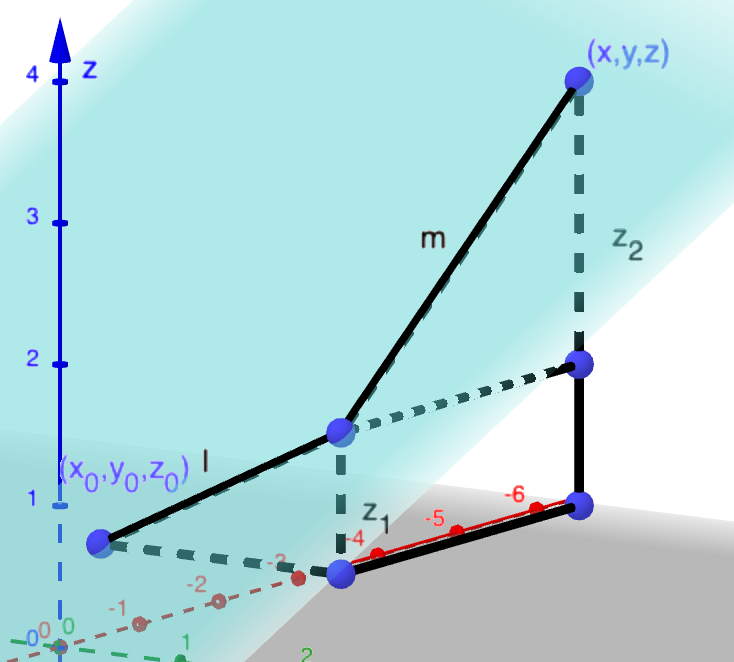
\includegraphics[scale=0.5]{skitser/tangent_plan.png}
\end{figure}

På skitsen er et plan, der følger linjerne $l$ og $m$.
Noterer vi hældningen af $l$ som $p$ og hældningen af $m$ som $q$,
så kan vi opstille følgende udtryk for ændringen på $z$-aksen:

$$
    \Delta z_1=p \cdot (x-x_0)
$$

$$
    \Delta z_2=q \cdot (y-y_0)
$$

Derfor må den nye funktionsværdi $z$ i punktet $(x,y,z)$ være:

$$
    z=z_0+\Delta z_1+\Delta z_2=p \cdot (x-x_0)+q \cdot (y-y_0) + z_0
$$

Det vil sige, at alle $(x,y,z)$, der gør nedenstående ligning sand, er punkter i planet tilhørende
linje $l$ og $m$ med afsæt i punkt $(x_0,y_0,z_0)$:

$$
z=p \cdot (x-x_0)+q \cdot (y-y_0) + z_0
$$

Det ovenstående er dog blot for det generelle plan.
For en tangent plan, som viser hældningen af en funktion af 2 variable,
kan hældningen langs $x$-aksen beskrives som $f_x'(x_0,y_0)$
og langs $y$-aksen $f_y'(x_0,y_0)$.
Sidst kan $z_0$ beskrives som $f(x_0,y_0)$, derfor:

$$
    z=f_x'(x_0,y_0)(x-x_0)+
    f_y'(x_0,y_0)(y-y_0)+
    f(x_0,y_0)
$$

Dette er ligningen for tangentplanet for en funktion af 2 variable.

\end{proofw}
